\chapter{Desenvolvimento}

\section{INTEGRAÇÃO ENTRE AS ENGENHARIAS DA FACULDADE DO GAMA – UnB}

Para a realização deste projeto é necessária uma conversa entre as cinco engenharias presentes na Faculdade do Gama da Universidade de Brasília, sendo elas: engenharia aeroespacial, engenharia automotiva, engenharia de energia, engenharia de software e engenharia eletrônica. 

A equipe foi separada por cursos, sendo que a área de automotiva e aeroespacial foram unidas por falta de pessoal das áreas para fazer equipes separadas. Essa primeira equipe ficou responsável pelo projeto mecânico e análise estrutural, pelos materiais, pelo acionamento do braço mecânico, pelos sensores, pelos desenhos das peças, pelo monitoramento, pelo projeto de fabricação e pelo controle do transdutor. A equipe de energia ficou responsável por encontrar as melhores fontes energéticas para o projeto, pelos materiais também, pela autonomia e consumo do aparelho e obviamente, a eficiência energética dele.
	
Já a equipe de software ficou responsável pela modelagem de requisitos gerais do projeto, pelo software embarcado, pela interface de usuário e pela comunicação crítica dos aparelhos em tempo real. E a equipe de eletrônica ficou responsável também pelo acionamento do parelho, pelos sensores, pelo processamento de sinais, pela eletrônica embarcada, pelo software embarcado também e controlo do transdutor juntamente com a equipe de aeroespacial e automotiva.

A conversa entre todas essas engenharias é de extrema importância, pois elas precisam estar andando juntas para que o projeto possa ser concluído e entregue sem falhas, e para isso testes serão necessários de todas as áreas, para que cada função ocorra como determinado.

\section{FERRAMENTAS DE TRABALHO E COMUNICAÇÃO}

\begin{itemize}
\item Comunicação da equipe geral e subequipes: SLACK e WHATSAPP
\item Ferramenta KANBAM: TRELLO
\item Ferramenta de repositório: GITHUB
\item Ferramenta de edição de texto do modelo Latex: TEXMAKER
\item Ferramenta CAD: CATIA V5R19 
\end{itemize}

\section{METODOLOGIA DE TRABALHO}

\subsection{METODOLOGIA GERAL}
A metodologia geral de trabalho de toda equipe ficou decidida como sendo reuniões dos gerentes de cada área com suas respectivas subequipes a fim de buscar ideias gerais, que depois seriam passadas para todos os gerentes para poderem filtrar as ideias e verem quais ideias conversavam melhor entre si para que fossem discutidas a melhor forma de usá-las no projeto e, dessa forma, os gerentes de cada área passarem as atividades a serem feitas para sua equipe. 

	Como ferramenta kanbam para a distribuição de atividades foi escolhido o trello, aonde as atividades foram distribuídas para cada um em forma de Sprint, os documentos gerados no trabalho foram para o repositório da turma no Github, epara a comunicação mais formal, direta e recebimentos das atividades do trello foi escolhido o slack e a comunicação mais informal foi o whatsapp, utilizado principalmente para dúvidas rápidas para não tirar o foco da comunicação do slack.

\subsection{METODOLOGIA DE CADA ÀREA}
A metodologia de trabalho da área de automotiva e aeroespacial foi determinada entre os membros dessa subequipe do projeto como sendo a divisão em dois grupos, o primeiro responsável pelo desenvolvimento do desenho do braço mecânico na ferramenta CAD e o segundo grupo ficou responsável pela a análise e escolha dos matérias que irão compor o braço.

	A subequipe de engenharia de energia do projeto, como conta com quatro membros, ficou definido como metodologia de trabalho entres os membros que cada um ficaria responsável por uma atividades, sendo elas: definição das fontes de energia, definição ada autonomia e consumo, definição da eficiência energética e definição dos materiais.
	
	A equipe de engenharia de software utilizou como metodologia, para definir os requisitos, a técnica de Brainstorming e buscou alinhar os requisitos levantados com os definidos pelas outras áreas e atuação do projeto. Após a definição dos requisitos a equipe foi dividida em duplas para buscar diferentes tecnologias que viabilizassem os requisitos definidos e por fim discutir a melhor solução.
	
	A equipe de engenharia eletrônica decidiu trabalhar dividindo os membros da sua subequipe em quatro grupos. O primeiro grupo ficou responsável pelo módulo controlador e os sinais emitidos por ele; o segundo grupo ficou responsável pelo módulo de transmissão e recebimento de dados de movimento e imagem; o terceiro ficou responsável pelo módulo de acoplamento do transdutor selecionado ao braço mecânico e o quarto grupo responsável pelo módulo eletrônico para o braço mecânico.	 

\section{REQUISITOS}

\subsection{REQUISITOS GERAIS}

\begin{itemize}
\item Braço mecânico leve e transportável;
\item Unidade de medição inercial para fácil manuseamento pelo profissional;
\item Uma fonte energética primária para o braço e outra secundária para segurança do paciente;
\item Boa rede de comunicação entre a unidade de medição inercial e braço para evitar grandes delays, utilizando captura de movimentos;
\item Transferência dos dados de movimento do braço mecânico e de imagens do sistema de ultrassom com baixa latência e alta qualidade;
\item Movimentação do braço feitas por um controlador central;
\item Aparelho de ultrassonografia;
\item Liberdade de movimentação do braço.
\end{itemize}

\subsection{REQUISITOS ESPECÍFICOS}

\begin{itemize}
\item Unidade de medição inercial confortável e de bom controle do braço mecânico;
\item Sensor óptico de distância para melhorar a exatidão dos movimentos do braço mecânico;
\item Suporte a internet cabeada de par trançado e, se disponível, fibra óptica;
\item Definição do sistema de ultrassom mais compatível com o projeto final e utilizado nos exames médicos mais frequentes;
\item Transferência das imagens geradas pelo sistema ultrassônico utilizando internet;
\item Duas janelas de transmissão de vídeo, uma correspondente ao ambiente do paciente e a outra correspondente a imagem gerada pela máquina de ultrassom;
\item Transmissão de vídeo realizada utilizando o Red5 server;
\item Servomotores para movimentação do braço;
\item Projeto e desenho técnico do braço em CAD;
\item Liberdade de movimentação do braço mecânico em translação e rotação;
\item Material do braço leve e que ofereça transportabilidade – alumínio;
\item Análise estrutural do projeto por meio de softwares específicos (ex: Ansys e Catia V5R19);
\item Análise normativa e de segurança do braço mecânico;
\item API para lidar com requisições HTTP e autenticação utilizando o framework Django REST;
\item Interface de sistema utilizando o framework Vue.js consumindo os dados da API;
\item Cadastro de médicos e unidades de ultrassom;
\item Geração de laudos online;
\item Servidor configurado utilizando o NGINX;
\item Sistema de Load Balacing para evitar atraso no processamento e fazer o tratamento de falhas;
\item Usuários autenticados antes da utilização;
\item Laudos gerados serão transmitidos a unidade de ultrassom criptografados de ponta-a-ponta, onde somente os usuários envolvidos terão acesso ao laudo.
\item Fonte primária de energia para o braço mecânico é alimentação pela tomada;
\item Fonte secundária do braço mecânico é uma bateria ligada a um sistema de placa fotovoltaica;
\item Fonte principal da unidade de medição inercial é a alimentação por tomada;
\item Fonte secundária da unidade de medição inercial é uma bateria;
\item A bateria de lítio para braço mecânico recarregável, visando algo mais ecológic; 
\item Bateria para supressão secundária para a unidade de medição inercial.
\end{itemize}

\subsection{REQUISITOS PRÁTICOS DO PROTÓTIPO}

\begin{itemize}
\item Altura aproximada do braço do protótipo de 30 centímetros;
\item Servomototres para movimentação do braço do protótipo;
\item Unicadade de medição inercial com acelerômetro e giroscópio integrados que seja compatível coma plataforma Arduino (sensor MPU-6050);
\item Programação do módulo controlador e servomotores para a plataforma Arduino;
\item Materiais de impressão 3D (ABS – acrilonitrila butadieno estireno e PETG – politereftalato de etileno glicol) para confecção do protótipo;
\item Impressora 3D;
\item Desenvolvimento dos softwares para o arduino;
\item Webcam segurada pelo braço;
\item Processamento e envio da imagem da webcam;
\item Bateria para o braço mecânico;
\item Dois computadores.
\end{itemize}

\section{ESTRUTURA ANALÍTICA DO PROJETO (EAP)}

\begin{figure}[h]
	\centering
	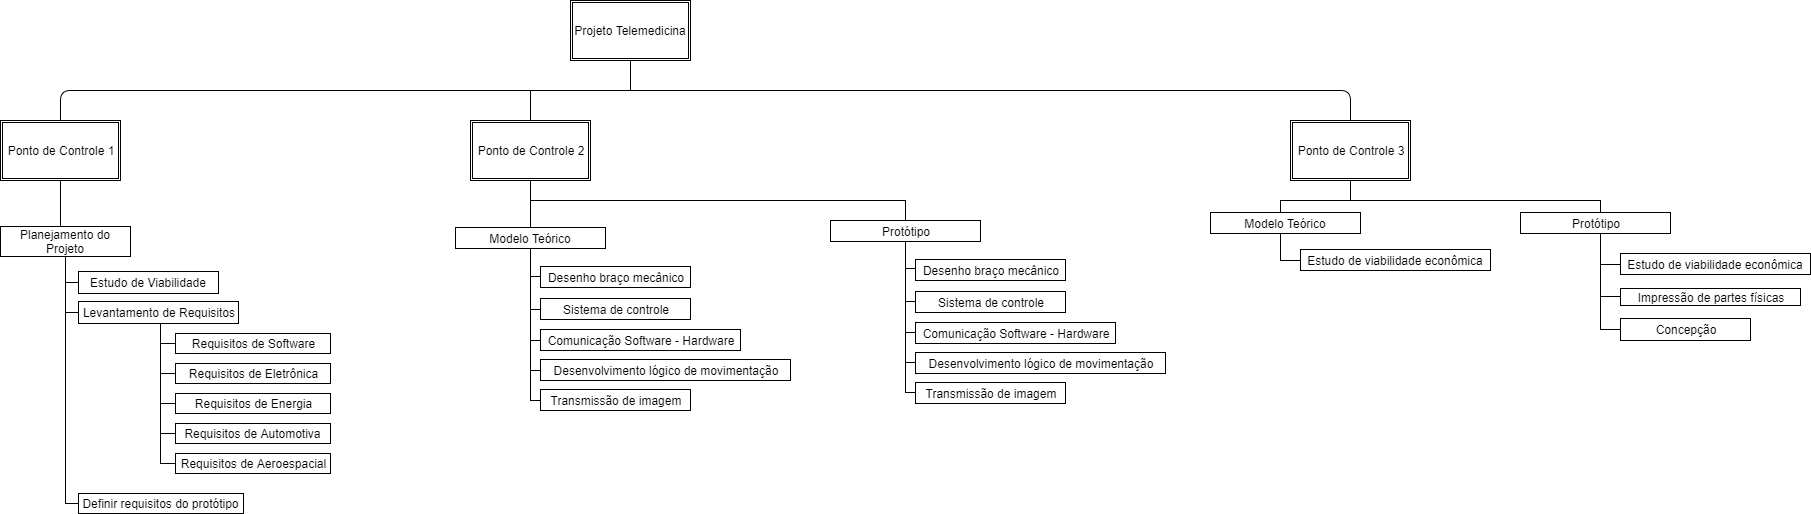
\includegraphics[keepaspectratio=true,scale=0.21]{figuras/eap_pi1.png}
	\caption{Estrutura analítica do projeto}
	\label{eap_fig01}
\end{figure}

Para melhor visualização, a figura \ref{eap_fig01} foi cortada e apresentada a seguir:

\begin{figure}[h]
\centering
\begin{minipage}[c]{\textwidth}
\centering
  		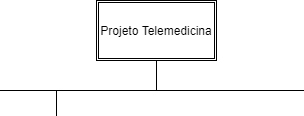
\includegraphics[scale=0.5]{figuras/eap_cort1.png} \\
  		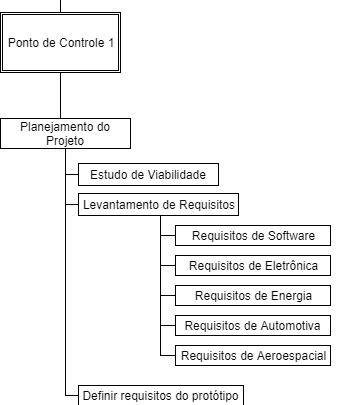
\includegraphics[scale=0.5]{figuras/eap_cort2.png} \\
  		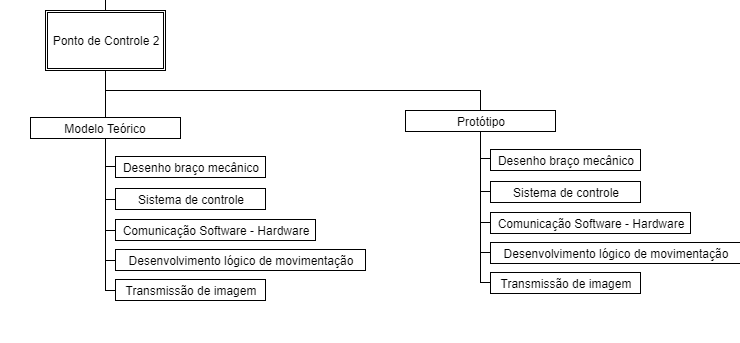
\includegraphics[scale=0.5]{figuras/eap_cort3.png} \\
 	    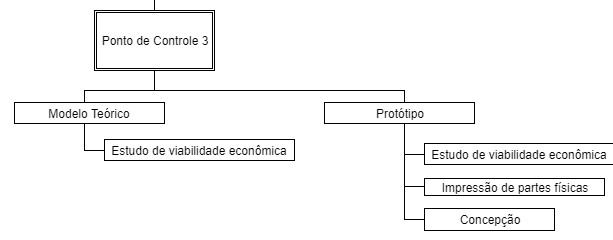
\includegraphics[scale=0.5]{figuras/eap_cort4.png}
    	\caption{Estrutura analítica do projeto repartida}
    	\label{fig:sample_figure}
\end{minipage}
\end{figure}


\section{MACRO CRONOGRAMA DO PROJETO}

\section*{Ponto de Controle 1)}
\begin{itemize}
\item Escolha das ferramentas de trabalho
\item Escolhas da metodologia de trabalho
\item Ideia do projeto definida
\item Definição do protótipo
\item Traçar os requisitos gerais, específico e do protótipo
\item EAP 
\item Macro cronograma
\end{itemize}

\section*{Ponto de Controle 2)}
\begin{itemize}
\item Desenhos do braço mecânico teórico e do protótipo
\item Desenhos ou Escolha da unidade de medição inercial ideal teórico e do protótipo
\item Determinação da comunicação software-eletrônica teórica e do protótipo
\item Desenhos de circuitos analógicos e digitais necessários teóricos e do protótipo
\item Desenvolvimento lógico de softwares para a movimentação teórica e do protótipo
\item Desenvolvimento do envio e recepção da imagem teórico e do protótipo
\item TESTES
\end{itemize}

\section*{Ponto de Controle 3)}
\begin{itemize}
\item Impressão do protótipo
\item Viabilidade econômica do produto teórico e do protótipo
\item Explicar as diferenças
\item Encerramento do Produto
\end{itemize}

\noindent\textit{Observação:} O macro cronograma pode sofrer alteração com o andamento do projeto durante o semestre.